\documentclass[preview]{standalone}
\usepackage{tkz-graph}
\begin{document}

\begin{figure}[ht]
\center
 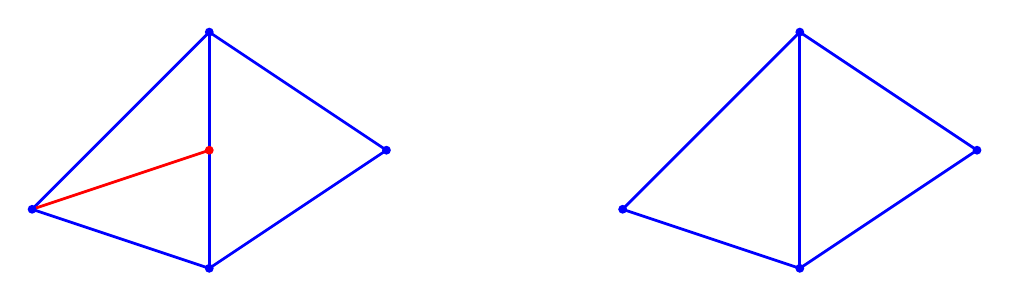
\begin{tikzpicture}[scale=0.75]

   \draw[color=blue,line width=1pt] (0,1) -- (3,0);
   \draw[color=blue,line width=1pt] (3,0) -- (3,4);
   \draw[color=blue,line width=1pt] (3,4) -- (0,1);
   \draw[color=blue,line width=1pt] (3,0) -- (6,2);
   \draw[color=blue,line width=1pt] (3,4) -- (6,2);
   \draw[color=red,line width=1pt] (0,1) -- (3,2);
   \fill [blue] (0,1) circle (0.075);
   \fill [blue] (3,0) circle (0.075);
   \fill [blue] (3,4) circle (0.075);
   \fill [blue] (6,2) circle (0.075);
   \fill [red] (3,2) circle (0.075);

   \draw[color=blue,line width=1pt] (10,1) -- (13,0);
   \draw[color=blue,line width=1pt] (13,0) -- (13,4);
   \draw[color=blue,line width=1pt] (13,4) -- (10,1);
   \draw[color=blue,line width=1pt] (13,0) -- (16,2);
   \draw[color=blue,line width=1pt] (13,4) -- (16,2);
   \fill [blue] (10,1) circle (0.075);
   \fill [blue] (13,0) circle (0.075);
   \fill [blue] (13,4) circle (0.075);
   \fill [blue] (16,2) circle (0.075);


 \end{tikzpicture}
\end{figure}





\end{document}



После: convert pdf to png
https://convertio.co/pdf-png/



 






